\exercisesheader{}

% 31

\eoce{\qt{Body measurements, Part IV\label{body_measurements_weight_height_inf}} 
The scatterplot and least squares summary below show the relationship 
between weight measured in kilograms and height measured in centimeters 
of 507 physically active individuals.

\noindent\begin{minipage}[c]{0.4\textwidth}
\begin{center}
\includegraphics[width=\textwidth]{ch_regr_simple_linear/figures/eoce/body_measurements_weight_height_inf/body_measurements_weight_height.pdf}
\end{center}
\end{minipage}
\begin{minipage}[c]{0.6\textwidth}
{\scriptsize
\begin{center}
\begin{tabular}{rrrrr}
    \hline
            & Estimate  & Std. Error    & t value   & Pr($>$$|$t$|$) \\ 
    \hline
(Intercept) & -105.0113 & 7.5394        & -13.93    & 0.0000 \\ 
height      & 1.0176    & 0.0440        & 23.13     & 0.0000 \\
    \hline
\end{tabular}
\end{center}
}
\end{minipage}
\begin{parts}
\item Describe the relationship between height and weight.
\item Write the equation of the regression line. Interpret the slope 
and intercept in context.
\item Do the data provide strong evidence that an increase in height 
is associated with an increase in weight? State the null and alternative 
hypotheses, report the p-value, and state your conclusion.
\item The correlation coefficient for height and weight is 0.72. 
Calculate $R^2$ and interpret it in context.
\end{parts}
}{}

% 32

\eoce{\qt{Beer and blood alcohol content\label{beer_blood_alcohol_inf}} 
Many people believe that gender, 
weight, drinking habits, and many other factors are much more important 
in predicting blood alcohol content (BAC) than simply considering the 
number of drinks a person consumed. Here we examine data from sixteen 
student volunteers at Ohio State University who each drank a randomly 
assigned number of cans of beer. These students were evenly divided 
between men and women, and they differed in weight and drinking habits. 
Thirty minutes later, a police officer measured their blood alcohol 
content (BAC) in grams of alcohol per deciliter of blood.
\footfullcite{Malkevitc+Lesser:2008} The scatterplot and regression 
table summarize the findings.

\noindent\begin{minipage}[c]{0.4\textwidth}
\begin{center}
\includegraphics[width=\textwidth]{ch_regr_simple_linear/figures/eoce/beer_blood_alcohol_inf/beer_blood_alcohol.pdf}
\end{center}
\end{minipage}
\begin{minipage}[c]{0.6\textwidth}
{\scriptsize
\begin{center}
\begin{tabular}{rrrrr}
    \hline
            & Estimate  & Std. Error    & t value   & Pr($>$$|$t$|$) \\ 
    \hline
(Intercept) & -0.0127   & 0.0126        & -1.00     & 0.3320 \\ 
beers       & 0.0180    & 0.0024        & 7.48      & 0.0000 \\ 
    \hline
\end{tabular}
\end{center}
}
\end{minipage}
\begin{parts}
\item Describe the relationship between the number of cans of beer 
and BAC.
\item Write the equation of the regression line. Interpret the slope 
and intercept in context.
\item Do the data provide strong evidence that drinking more cans of 
beer is associated with an increase in blood alcohol? State the null 
and alternative hypotheses, report the p-value, and state your 
conclusion.
\item The correlation coefficient for number of cans of beer and BAC 
is 0.89. Calculate $R^2$ and interpret it in context.
\item Suppose we visit a bar, ask people how many drinks they have had, 
and also take their BAC. Do you think the relationship between number 
of drinks and BAC would be as strong as the relationship found in the 
Ohio State study?
\end{parts}
}{}

% 33

\eoce{\qt{Husbands and wives, Part II\label{husbands_wives_height_inf}} The 
scatterplot below summarizes husbands' and wives' heights in a random 
sample of 170 married couples in Britain, where both partners' ages are 
below 65 years. Summary output of the least squares fit for predicting 
wife's height from husband's height is also provided in the table.

\noindent\begin{minipage}[c]{0.4\textwidth}
\begin{center}
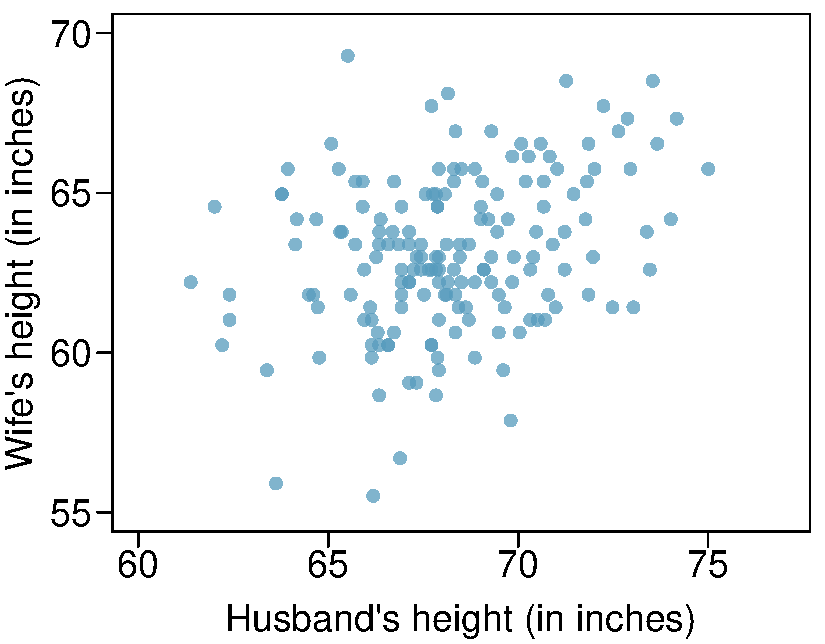
\includegraphics[width=\textwidth]{ch_regr_simple_linear/figures/eoce/husbands_wives_height_inf_2s/husbands_wives_height_inf_2s}
\end{center}
\end{minipage}
\begin{minipage}[c]{0.6\textwidth}
{\scriptsize
\begin{center}
\begin{tabular}{rrrrr}
    \hline
                    & Estimate  & Std. Error    & t value   & Pr($>$$|$t$|$) \\ 
    \hline
(Intercept)         & 43.5755   & 4.6842        & 9.30      & 0.0000 \\ 
height\_\hspace{0.3mm}husband   & 0.2863    & 0.0686        & 4.17      & 0.0000 \\ 
    \hline
\end{tabular}
\end{center}
}
\end{minipage}
\begin{parts}
\item Is there strong evidence that taller men marry taller women? 
State the hypotheses and include any information used to conduct the test.
\item Write the equation of the regression line for predicting wife's 
height from husband's height.
\item Interpret the slope and intercept in the context of the application.
\item Given that $R^2 = 0.09$, what is the correlation of heights 
in this data set?
\item You meet a married man from Britain who is 5'9" (69 inches). 
What would you predict his wife's height to be? How reliable is this 
prediction?
\item You meet another married man from Britain who is 6'7" (79 inches). 
Would it be wise to use the same linear model to predict his wife's 
height? Why or why not?
\end{parts}
}{}

% 34

\eoce{\qt{Urban homeowners, Part II\label{urban_homeowners_cond}}
Exercise~\ref{urban_homeowners_outlier} gives a scatterplot displaying the 
relationship between the percent of families that own their home and 
the percent of the population living in urban areas. Below is a 
similar scatterplot, excluding District of Columbia, as well as the 
residuals plot. There were 51 cases.

\noindent\begin{minipage}[c]{0.45\textwidth}
{\raggedright\begin{parts}
\item For these data, $R^2=0.28$. What is the correlation? How can 
you tell if it is positive or negative?
\item Examine the residual plot. What do you observe? Is a simple 
least squares fit appropriate for these data?
\end{parts}\vspace{15mm}}
\end{minipage}
\begin{minipage}[c]{0.1\textwidth}
$\:$ \\
\end{minipage}
\begin{minipage}[c]{0.43\textwidth}
\begin{center}
\includegraphics[width=\textwidth]{ch_regr_simple_linear/figures/eoce/urban_homeowners_cond/urban_homeowners_cond.pdf}
\end{center}
\end{minipage}
}{}

% 35

\eoce{\qt{Murders and poverty, Part II\label{murders_poverty_inf}}
Exercise~\ref{murders_poverty_reg} presents regression output from a model 
for predicting annual murders per million from percentage living in 
poverty based on a random sample of 20 metropolitan areas. The model 
output is also provided below.
\begin{center}
\begin{tabular}{rrrrr}
    \hline
            & Estimate  & Std. Error    & t value   & Pr($>$$|$t$|$) \\ 
    \hline
(Intercept) & -29.901   & 7.789         & -3.839    & 0.001 \\ 
poverty\%   & 2.559     & 0.390         & 6.562     & 0.000 \\ 
    \hline
\end{tabular}
\[ s = 5.512 \qquad R^2 = 70.52\% \qquad R^2_{adj} = 68.89\% \]
\end{center}
\begin{parts}
\item What are the hypotheses for evaluating whether poverty percentage 
is a significant predictor of murder rate?
\item State the conclusion of the hypothesis test from part (a) in 
context of the data.
\item Calculate a 95\% confidence interval for the slope of poverty 
percentage, and interpret it in context of the data.
\item Do your results from the hypothesis test and the confidence 
interval agree? Explain.
\end{parts}
}{}

% 36

\eoce{\qt{Babies\label{babies_head_gestation_inf}} Is the gestational age 
(time between conception and birth) of a low birth-weight baby useful 
in predicting head circumference at birth? Twenty-five low birth-weight 
babies were studied at a Harvard teaching hospital; the investigators 
calculated the regression of head circumference (measured in centimeters) 
against gestational age (measured in weeks). The estimated regression 
line is
\[ \widehat{head~circumference} = 3.91 + 0.78 \times gestational~age \]
\begin{parts}
\item What is the predicted head circumference for a baby whose 
gestational age is 28 weeks?
\item The standard error for the coefficient of gestational age is 0.
35, which is associated with $df=23$. Does the model provide strong 
evidence that gestational age is significantly associated with head 
circumference?
\end{parts} 
}{}
